\clearpage
\title{Finding root of nonlinear equation using Newton-Raphson Method.}
\author{}
\date{}
\maketitle

\section*{Introduction}

\subsection*{Newton-Raphson Method}
Newton Raphson Method is an open method and starts with one initial guess for finding real root of non-linear equations.\\\\
In Newton Raphson method if $a$ is initial guess then next approximated root $b$ is obtained by following formula:
\[b = a - \frac{f(a)}{f^\prime(a)}\]
From the above equation, we get the $x$ intersect of the slope at point $(a, f(a))$. Repeating this process get this point closer and closer to real root of the non-linear equation.\cite{prs}

\section*{Tools Used}
\begin{itemize}
    \item MATLAB R2021a - for writing and running code.
    \item MacTeX -\LaTeX  compiler.
    \item VS Code with \LaTeX workshop extension as a text editor.
\end{itemize}

\section*{Process}

\subsection*{Code for Newton-Raphson:}
\begin{minted}[breaklines, linenos]{matlab}
    
% Clearing Screen
clc

% Setting x as symbolic variable
syms x;

% Input Section
eqn = input('Enter non-linear equations: ');
a = input('Enter initial guess: ');
e = input('Tolerable error: ');
N = input('Enter maximum number of steps: ');

% Initializing step counter
step = 1;

% Finding derivate of given function
g = diff(eqn,x);

% Finding Functional Value
fa = eval(subs(eqn,x,a));

while abs(fa)> e
    fa = eval(subs(eqn,x,a));
    ga = eval(subs(g,x,a));
    if ga == 0
        disp('Division by zero.');
        break;
    end
    
    b = a - fa/ga;
    fprintf('step=%d\ta=%f\tf(a)=%f\n',step,a,fa);
    a = b;
    
    if step>N
       disp('Not convergent'); 
       break;
    end
    step = step + 1;
end

fprintf('Root is %f\n', a);
\end{minted}



\vspace{20mm}
\subsection*{Output}
\begin{center}
    \centering
    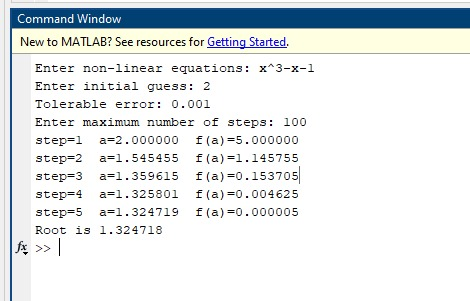
\includegraphics[width = .9\textwidth]{newar.jpeg}
    \captionof{figure}{Newton-Raphson method}
\end{center}

